\chapter{RESULTS}
\label{ch:results}

This chapter presents the results gathered by the simulations explained in chapter \ref{ch:simulation}. Three different sets of comparisons are presented. The first comparison shows the difference in accuracy of using a GPS sensor and a GPS coupled with a camera. The second case is to show how the delays affect the accuracy of the estimations. And the last case compares the estimations of the Extended Kalman filter against the Delayed Extended Kalman filter with delayed measurements, to see the impact of disregarding the delays.

\section{Comparison of Estimations Between GPS and GPS Coupled with Camera}
In this scenario, we focus on the comparison between using a GPS at 1 Hz coupled with a camera at 20 Hz, and the GPS alone. The introduction of the camera measurements are expected to improve the estimation. In this case, the GPS measurements have a random delay of 0.75 seconds.
%The first case uses one GPS sensor in the UAS with a frequency of 4 Hz. The measurement is assumed to be received instantaneously. This situation is not real but it is going to be simulated for the purpose of comparison and to recognize the impact that delays have in the estimates.
\begin{figure}[H]
  \centering
  \includegraphics[scale=0.40]{./Results/GPS_vs_GPS+Cam/uav_trajectory.eps}
  \caption[UAV Trajectory Comparison - GPS vs GPS and Camera]{UAV Trajectory Comparison - GPS vs GPS and Camera. The real trajectory of the aircraft is shown in this plot, against the estimated trajectory calculated by using a GPS coupled with a camera, and just a GPS.}
\end{figure}

\begin{figure}[H]
  \centering
  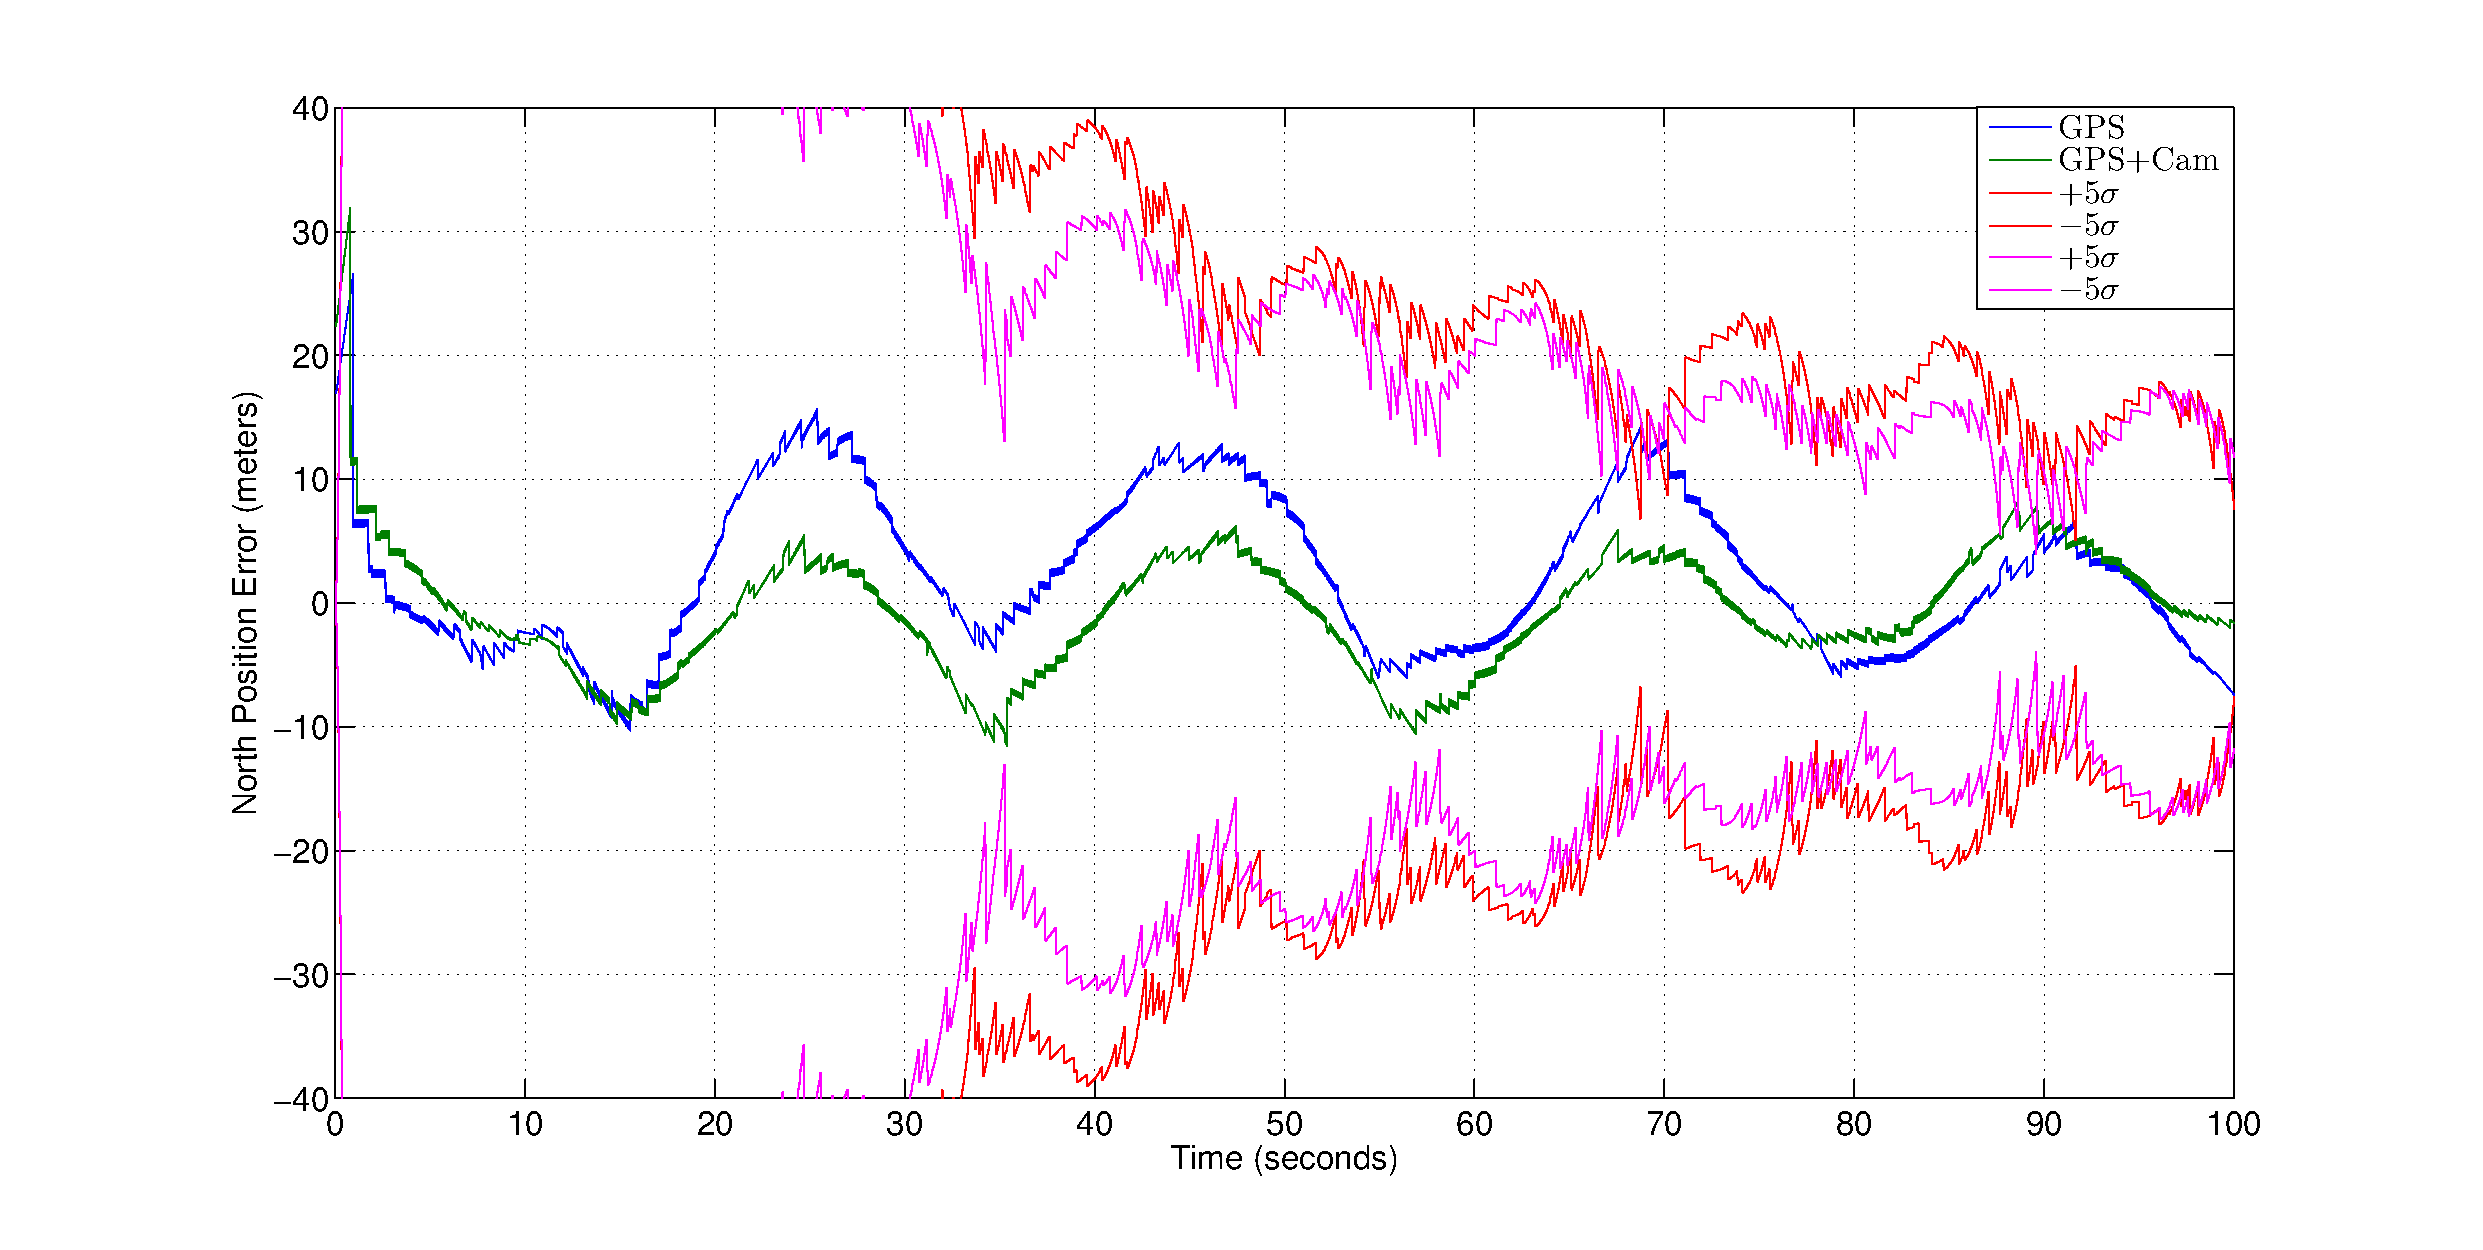
\includegraphics[scale=0.40]{./Results/GPS_vs_GPS+Cam/north_comparison.eps}
  \caption[North Position Error Comparison - GPS vs GPS and Camera]{North Position Error Comparison - GPS vs GPS and Camera. The error in the north position is shown in this plot. The states estimations are compared for GPS and GPS coupled with a camera.}
\end{figure}

\begin{figure}[H]
  \centering
  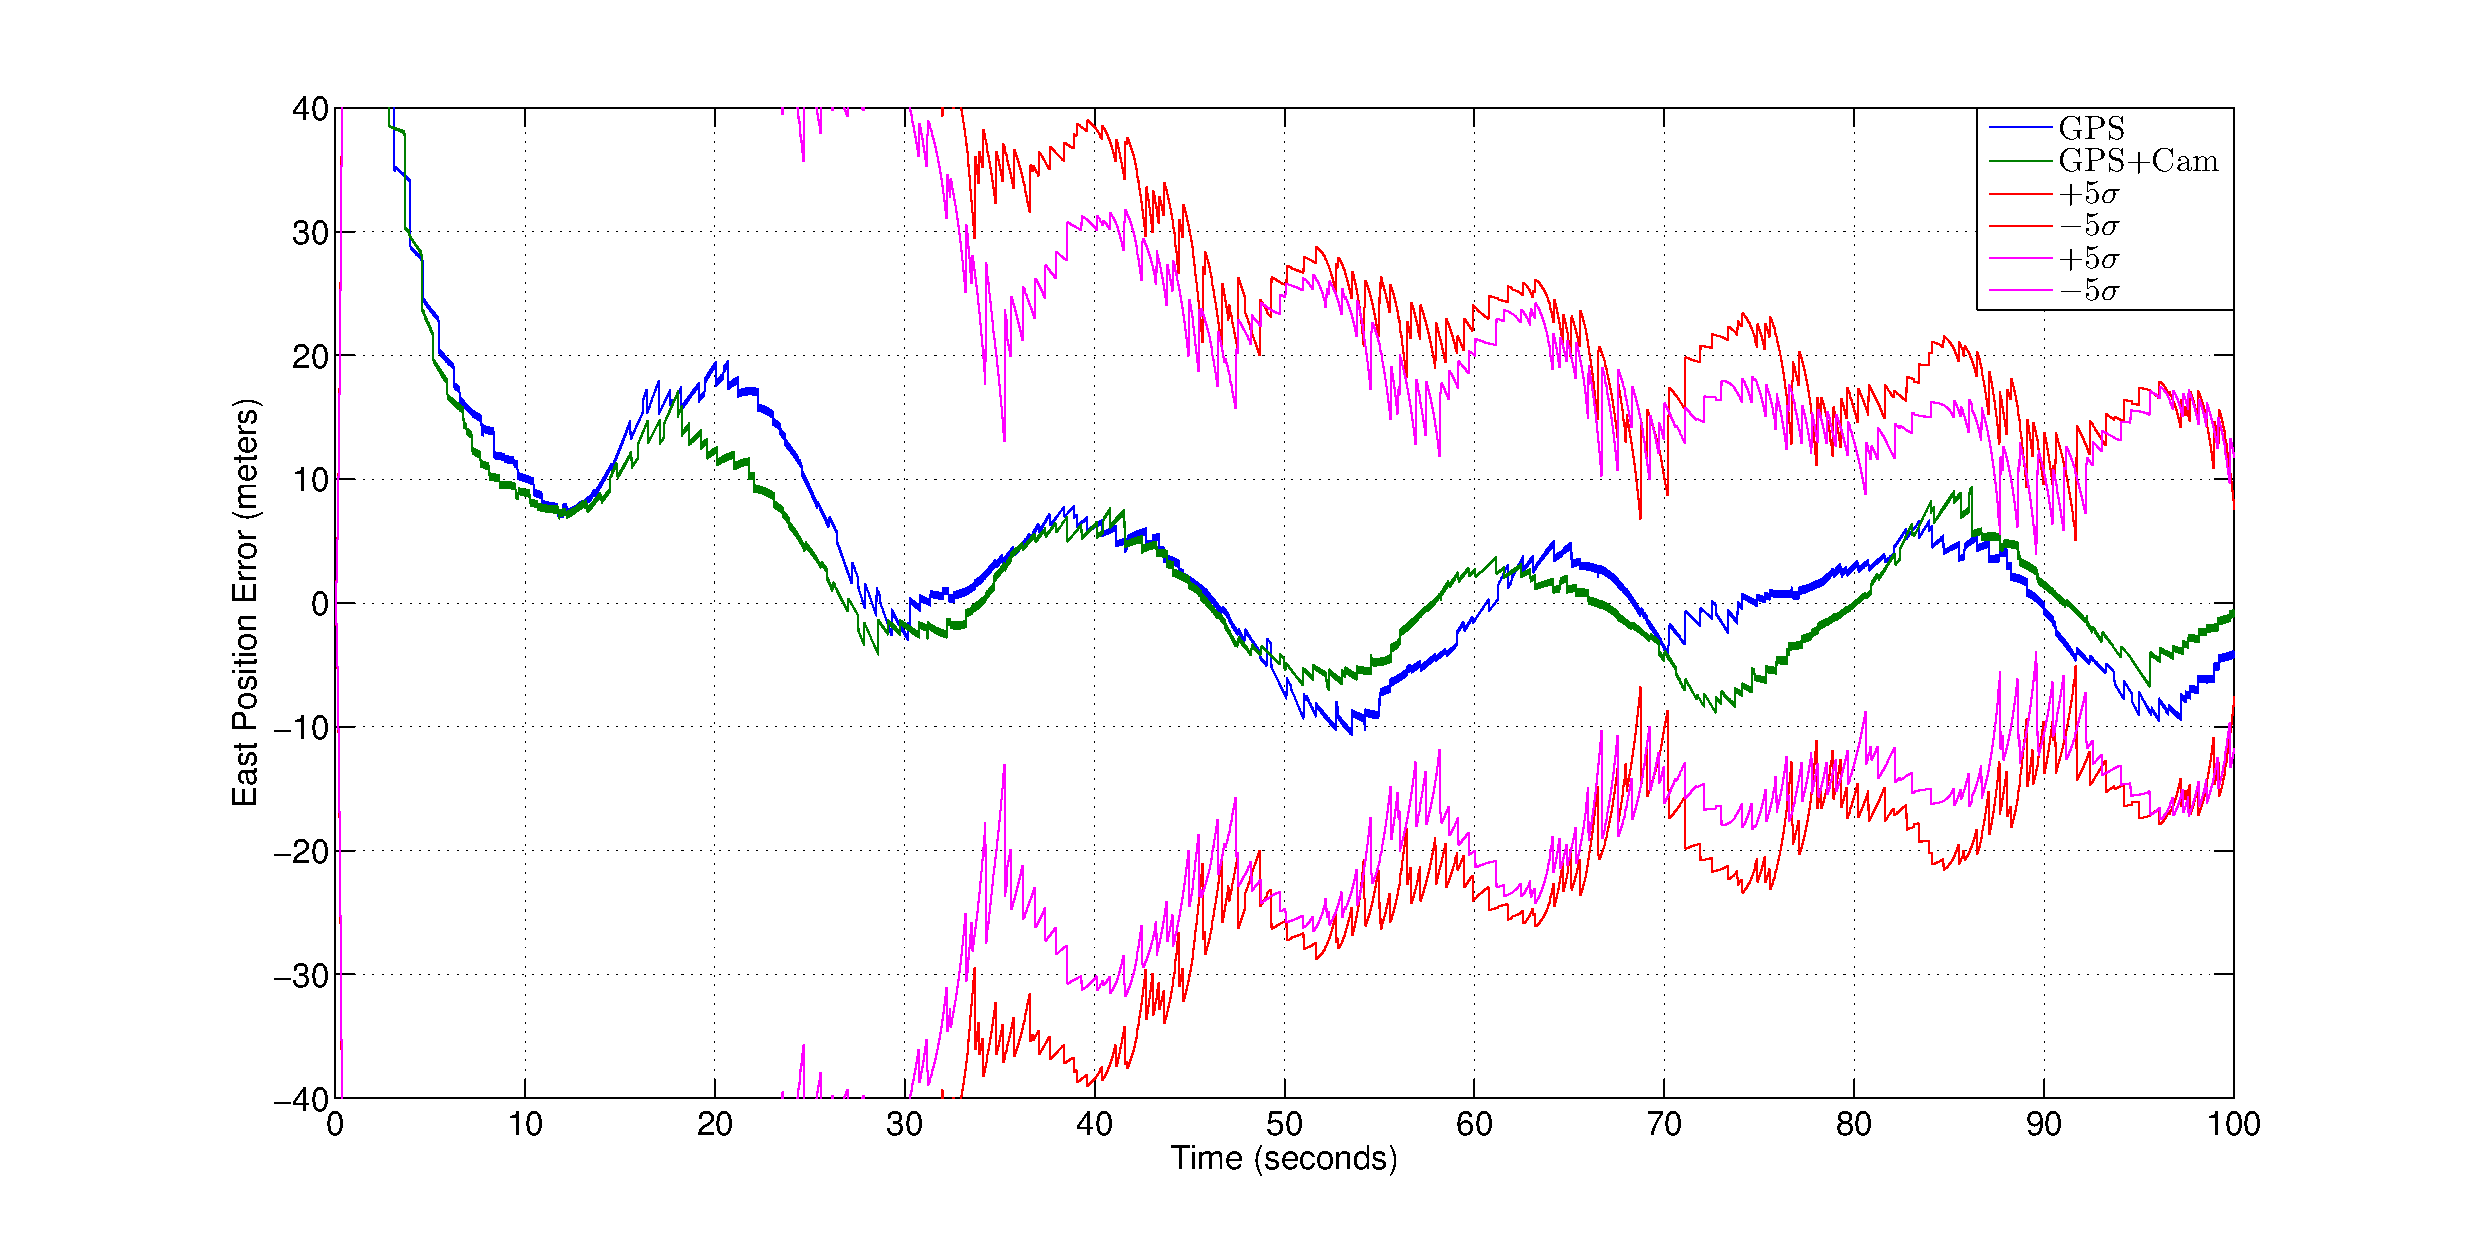
\includegraphics[scale=0.40]{./Results/GPS_vs_GPS+Cam/east_comparison.eps}
  \caption[East Position Error Comparison - GPS vs GPS and Camera]{East Position Error Comparison - GPS vs GPS and Camera. The error in the east position is shown in this plot. The states estimations are compared for GPS and GPS coupled with a camera.}
\end{figure}

\begin{figure}[H]
  \centering
  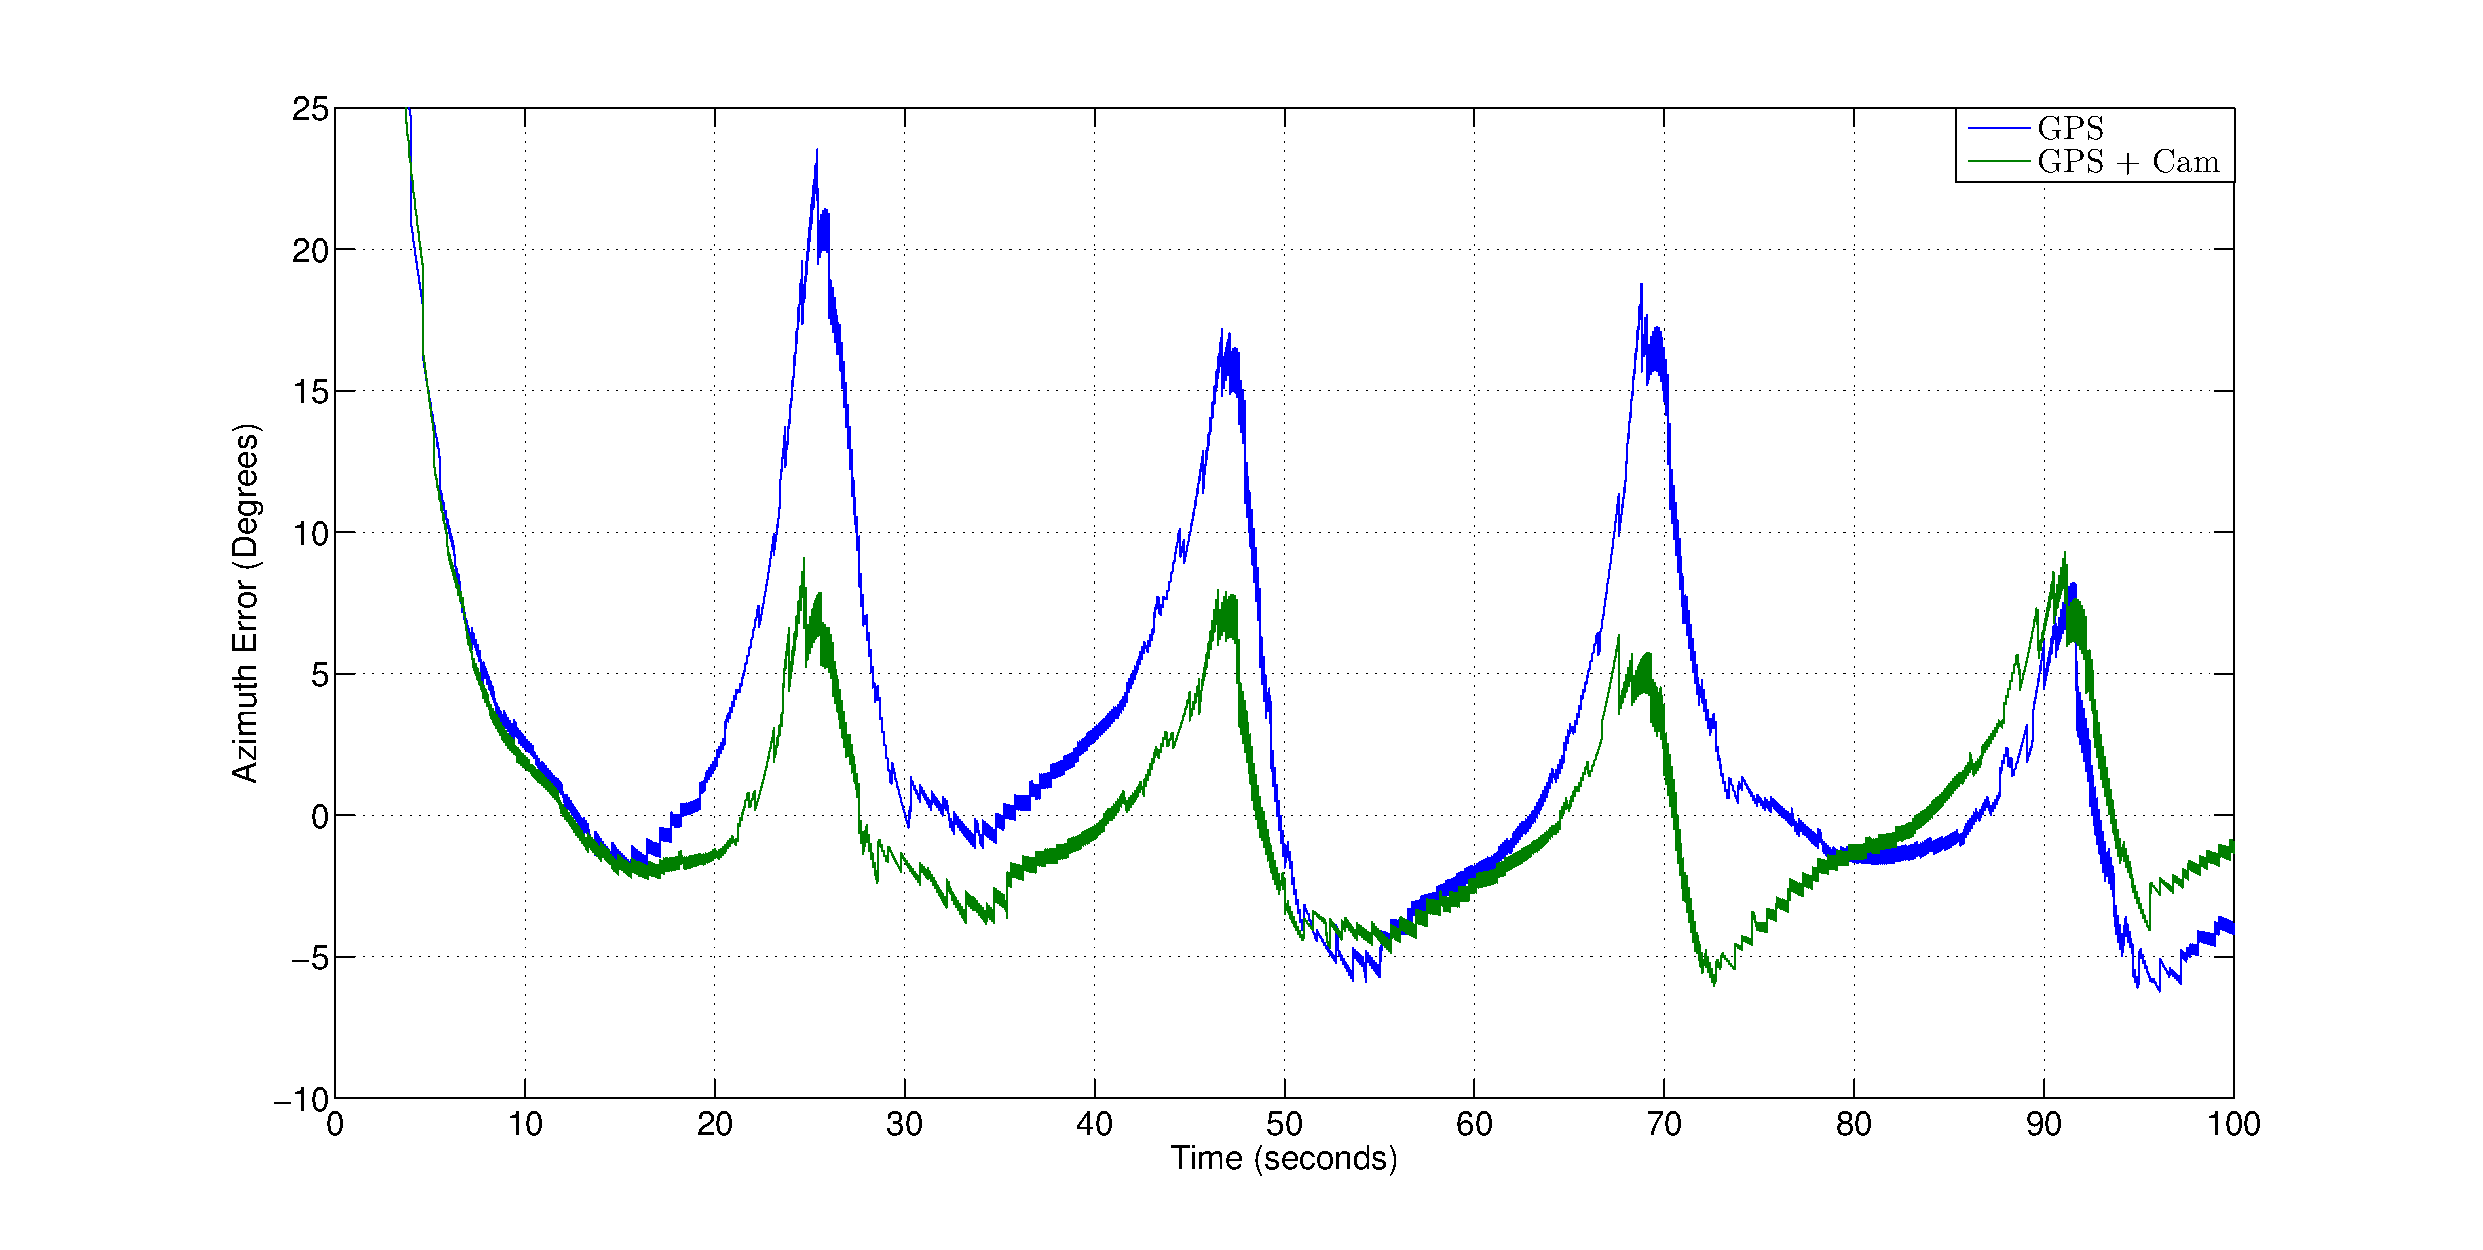
\includegraphics[scale=0.40]{./Results/GPS_vs_GPS+Cam/azimuth_comparison.eps}
  \caption[Azimuth Error Comparison - GPS vs GPS coupled with Camera]{Azimuth Error Comparison - GPS vs GPS coupled with Camera. The error in the azimuth angle calculated by the estimations are presented. It can be seen that coupling a GPS with a camera improves the estimation.}
\end{figure}
\begin{figure}[H]
  \centering
  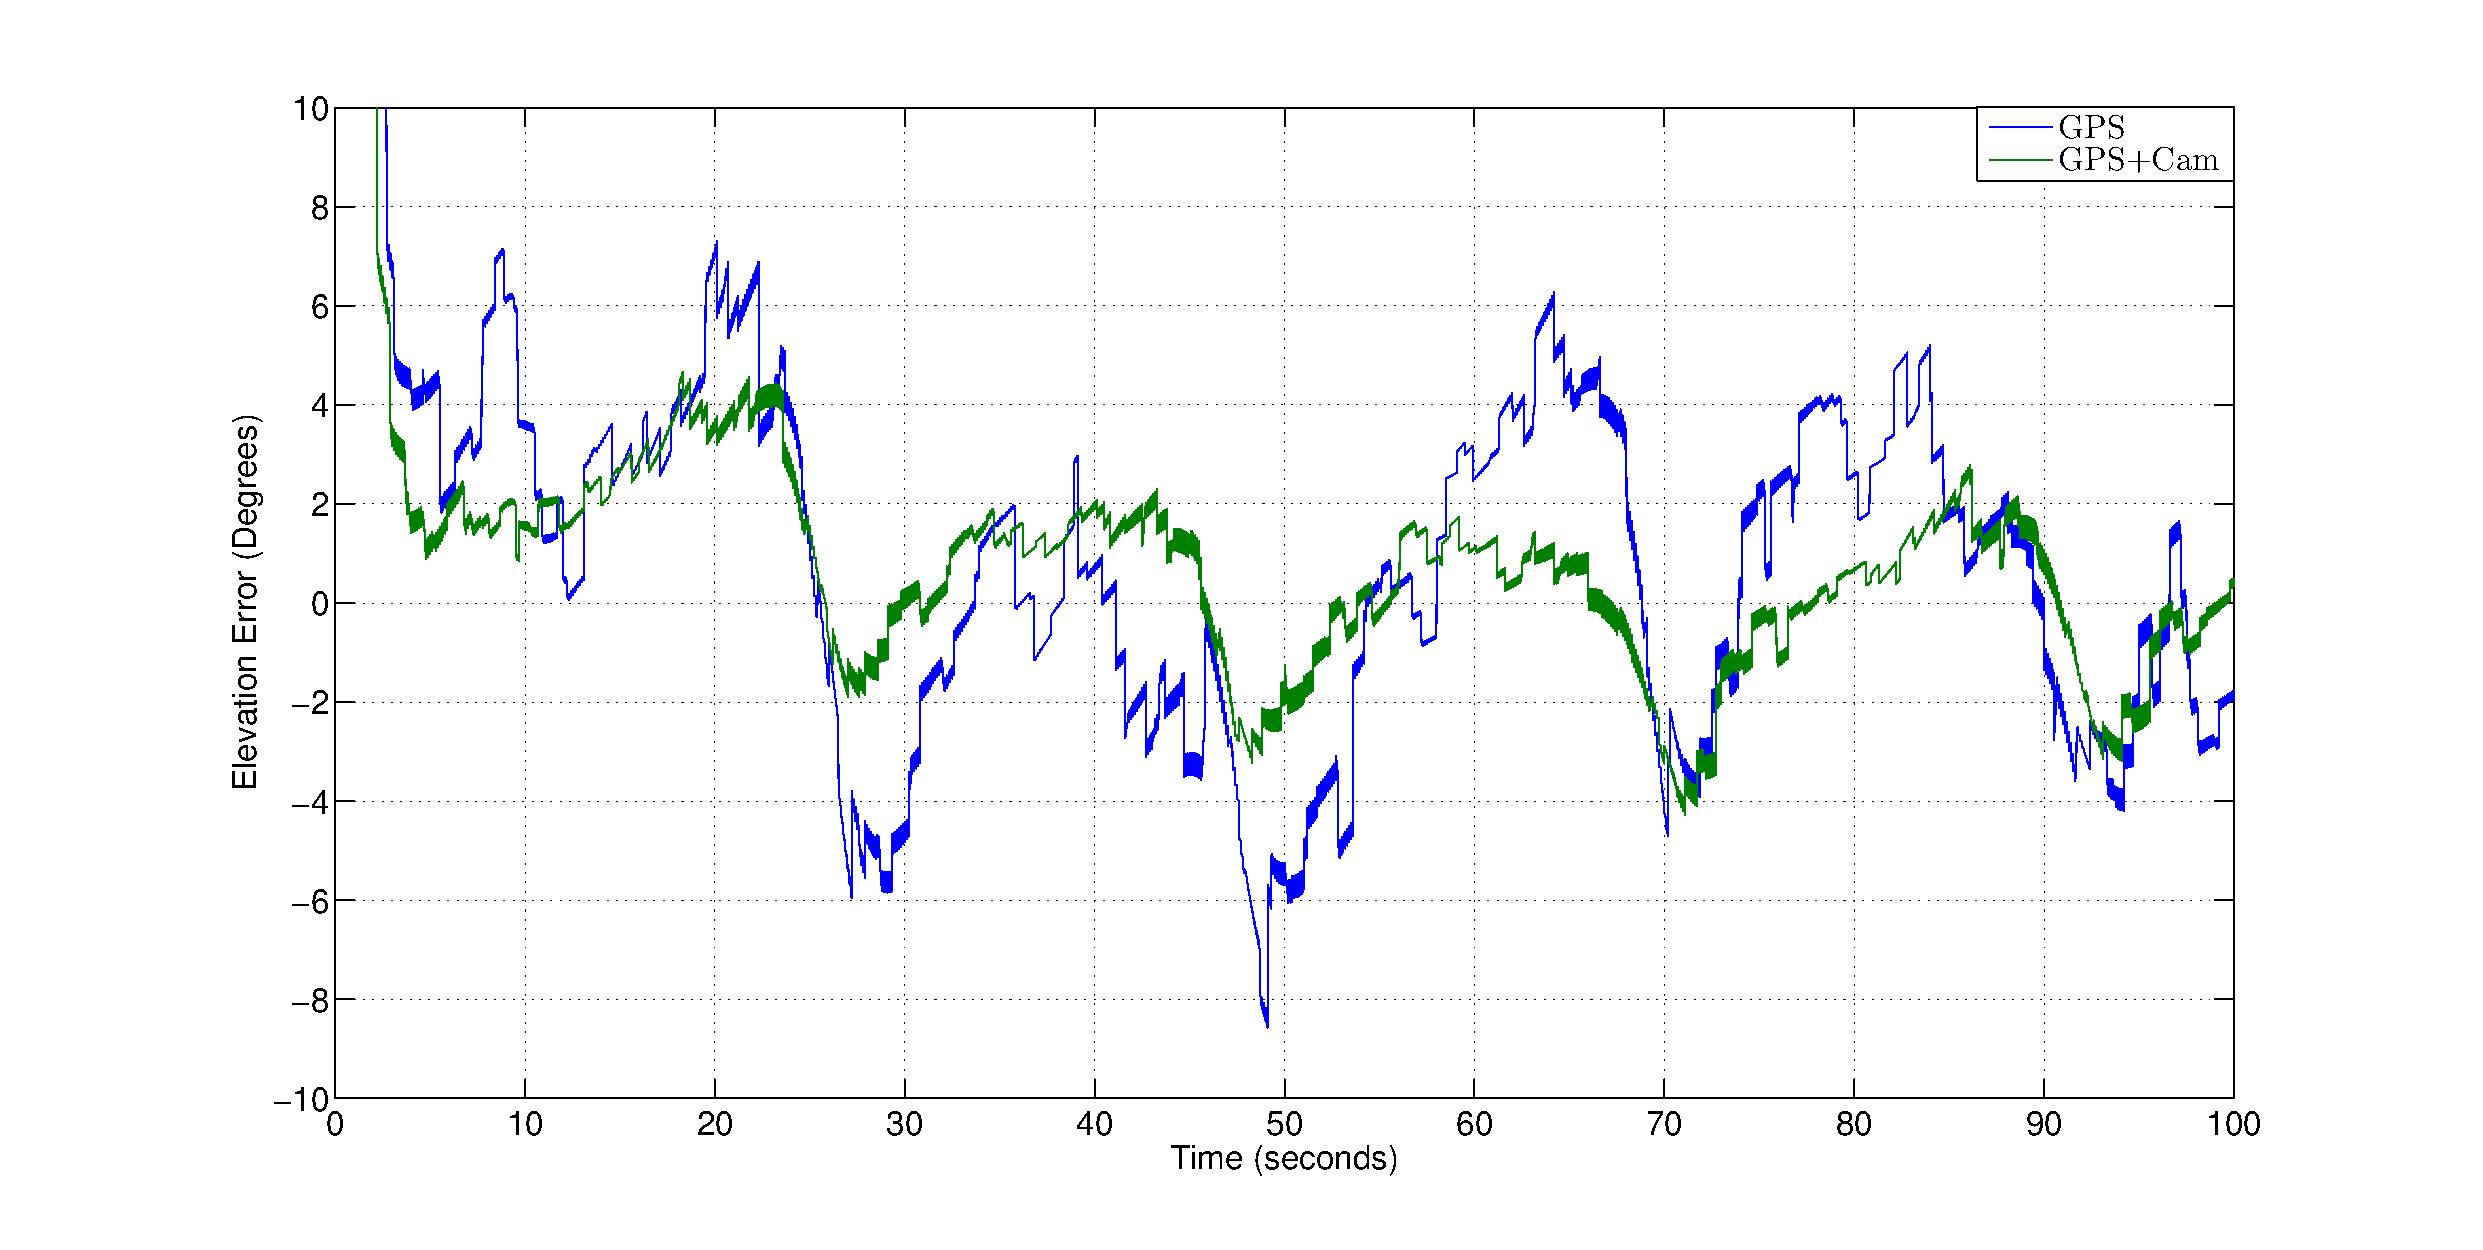
\includegraphics[scale=0.40]{./Results/GPS_vs_GPS+Cam/elevation_comparison.eps}
  \caption[Elevation Error Comparison - GPS vs GPS coupled with Camera]{Elevation Error Comparison - GPS vs GPS coupled with Camera. The error in the elevation angle calculated by the estimations are presented. It can be seen that coupling a GPS with a camera improves the estimation.}
\end{figure}

\pagebreak

\section{Comparison of Estimation Accuracy for EKF and DEKF with 0.75 s Random Delay}
In this scenario the precision of the state estimations from an EKF and a DEKF are considered. Again, a GPS coupled with a camera serves as the inputs for the filters. Here we show how the estimations are impacted if the measurements have delays and a filter that does not take them into account is used. An improvement in the estimations is expected using the DEKF.

\begin{figure}[H]
  \centering
  \includegraphics[scale=0.55]{./Results/EKF_vs_DEKF/uav_trajectory.eps}
  \caption[UAV Trajectory Comparison - EKF vs DEKF]{UAV Trajectory Comparison - EKF vs DEKF. The trajectory of the aircraft is shown in this plot, against the estimated trajectory calculated by an EKF and by a DEKF.}
\end{figure}

\begin{figure}[H]
  \centering
  \includegraphics[scale=0.40]{./Results/EKF_vs_DEKF/north_error_comparison.eps}
  \caption[North Position Error Comparison - EKF vs DEKF]{North Position Error Comparison - EKF vs DEKF. The error in the north position is shown in this plot. The states estimations are compared for an EKF and a DEKF.}
\end{figure}

\begin{figure}[H]
  \centering
  \includegraphics[scale=0.40]{./Results/EKF_vs_DEKF/east_error_comparison.eps}
  \caption[East Position Error Comparison - EKF vs DEKF]{East Position Error Comparison - EKF vs DEKF. The error in the east position is shown in this plot. The states estimations are compared for an EKF and a DEKF.}
\end{figure}

\begin{figure}[H]
  \centering
  \includegraphics[scale=0.40]{./Results/EKF_vs_DEKF/azimuth_error_comparison.eps}
  \caption[Azimuth Error Comparison - EKF vs DEKF]{Azimuth Error Comparison - EKF vs DEKF. The error in the azimuth angle calculated by the estimations is shown in this plot. Azimuth for the EKF and the DEKF are compared.}
\end{figure}

\begin{figure}[H]
  \centering
  \includegraphics[scale=0.40]{./Results/EKF_vs_DEKF/elevation_error_comparison.eps}
  \caption[Elevation Error Comparison - EKF vs DEKF]{Elevation Error Comparison - EKF vs DEKF. The error in the elevation angle calculated by the estimations is shown in this plot. Elevation for the EKF and the DEKF are compared.}
\end{figure}

\section{Comparison of Estimation Accuracy Between No delay, 0.25 s, 0.50 s, and 0.75 s Random Delays}
For this scenario we will use a GPS coupled with a camera. This scenario compares the estimation made by a DEKF for no delay, random delay of up to 0.25 s, 0.50 s, and 0.75 s. Since the delays are randomly generated, some of the measurements arrive in an out-of-sequence fashion. The Delayed Extended Kalman filter also compensates for this.

%This configuration uses a GPS sensor at 4 Hz coupled with a camera at 10 Hz. As explained before, the reason for this configuration comes from the nature of each sensor. The GPS has relative low error at medium and long distance but not at close range. Inversely, the camera is faster than the GPS and makes good estimations at short distances, but at medium and long range it can not detect the target. Hence, the sensors complement each other.

\begin{figure}[H]
  \centering
  \includegraphics[scale=0.55]{./Results/Delay_Comparison/uav_trajectory.eps}
  \caption[UAV Trajectory Comparison - Different Delays]{UAV Trajectory Comparison - Different Delays. The trajectory of the aircraft is shown in this plot, against the estimated trajectory calculated by a DEKF for no delay, 0.25 s, 0.50 s, and 0.75 s of random delay.}
\end{figure}

\begin{figure}[H]
  \centering
  \includegraphics[scale=0.40]{./Results/Delay_Comparison/north_error_comparison.eps}
  \caption[North Position Error Comparison - Different Delays]{North Position Error Comparison - Different Delays. The error in the north position is shown in this plot. The states estimations are compared for no delay, 0.25 s, 0.50 s, and 0.75 s of random delay.}
\end{figure}
\begin{figure}[H]
  \centering
  \includegraphics[scale=0.40]{./Results/Delay_Comparison/east_error_comparison.eps}
  \caption[East Position Error Comparison - Different Delays]{East Position Error Comparison - Different Delays. The error in the east position is shown in this plot. The states estimations are compared for no delay, 0.25 s, 0.50 s, and 0.75 s of random delay.}
\end{figure}

\begin{figure}[H]
  \centering
  \includegraphics[scale=0.40]{./Results/Delay_Comparison/azimuth_error_comparison.eps}
  \caption[Azimuth Error Comparison - Different Delays]{Azimuth Error Comparison - Different Delays. The error in the azimuth angle calculated by the estimations is shown in this plot. Azimuth for no delay, 0.25 s, 0.50 s, and 0.75 s of random delay, are compared.}
\end{figure}

\begin{figure}[H]
  \centering
  \includegraphics[scale=0.40]{./Results/Delay_Comparison/elevation_error_comparison.eps}
  \caption[Elevation Error Comparison - Different Delays]{Elevation Error Comparison - Different Delays. The error in the elevation angle calculated by the estimations is shown in this plot. Elevation for no delay, 0.25 s, 0.50 s, and 0.75 s of random delay, are compared.}
\end{figure}

%
%\subsection{Case 3 - GPS Sensor With Fixed Delay of 0.25 sec} \hspace{0pt} \\
%In this case, all the measurements are delayed 0.25 s. The delayed extended Kalman filter is used from now on.
%
%\begin{figure}[h!]
%  \centering
%  \includegraphics[scale=0.6]{./GPS/fixed_delay_0.25/fig4}
%  \caption{Real States vs Estimated States - Case 3}
%\end{figure}
%\pagebreak
%\begin{figure}[h!]
%  \centering
%  \includegraphics[scale=0.6]{./GPS/fixed_delay_0.25/fig5}
%  \caption{North Position Error - Case 3}
%\end{figure}
%\begin{figure}[h!]
%  \centering
%  \includegraphics[scale=0.6]{./GPS/fixed_delay_0.25/fig6}
%  \caption{East Position Error - Case 3}
%  \label{fig:theFig}
%\end{figure}
%\begin{figure}[h!]
%  \centering
%  \includegraphics[scale=0.6]{./GPS/fixed_delay_0.25/fig7}
%  \caption{GPS Position Error - Case 3}
%  \label{fig:theFig}
%\end{figure}
%
%\begin{figure}[h!]
%  \centering
%  \includegraphics[scale=0.6]{./GPS/fixed_delay_0.25/fig8}
%  \caption{Desired Azimuth vs Estimated Azimuth - Case 3}
%  \label{fig:theFig}
%\end{figure}
%\begin{figure}[h!]
%  \centering
%  \includegraphics[scale=0.6]{./GPS/fixed_delay_0.25/fig9}
%  \caption{Azimuth Error - Case 3}
%  \label{fig:theFig}
%\end{figure}
%\begin{figure}[h!]
%  \centering
%  \includegraphics[scale=0.6]{./GPS/fixed_delay_0.25/fig10}
%  \caption{Desired Elevation vs Estimated Elevation - Case 3}
%  \label{fig:theFig}
%\end{figure}
%\begin{figure}[h!]
%  \centering
%  \includegraphics[scale=0.6]{./GPS/fixed_delay_0.25/fig11}
%  \caption{Elevation Error - Case 3}
%  \label{fig:theFig}
%\end{figure}
%\begin{figure}[h!]
%  \centering
%  \includegraphics[scale=0.6]{./GPS/fixed_delay_0.25/fig12}
%  \caption{Normalized Azimuth and Elevation Errors - Case 3}
%  \label{fig:theFig}
%\end{figure}
%
%\subsection{Case 4 - GPS Sensor With Fixed Delay of 0.25 sec Disregarding Delay} \hspace{0pt} \\
%In this case, all the measurements are delayed 0.25 s. The difference is that a regular Extended Kalman filter is used, that means that the delays are not taking into account in the filter. This is done for comparison purposes.
%
%\begin{figure}[h!]
%  \centering
%  \includegraphics[scale=0.6]{./GPS_EKF/fixed_delay_0.25/fig4}
%  \caption{Real States vs Estimated States - Case 4}
%\end{figure}
%\pagebreak
%\begin{figure}[h!]
%  \centering
%  \includegraphics[scale=0.6]{./GPS_EKF/fixed_delay_0.25/fig5}
%  \caption{North Position Error - Case 4}
%\end{figure}
%\begin{figure}[h!]
%  \centering
%  \includegraphics[scale=0.6]{./GPS_EKF/fixed_delay_0.25/fig6}
%  \caption{East Position Error - Case 4}
%  \label{fig:theFig}
%\end{figure}
%\begin{figure}[h!]
%  \centering
%  \includegraphics[scale=0.6]{./GPS_EKF/fixed_delay_0.25/fig7}
%  \caption{GPS Position Error - Case 4}
%  \label{fig:theFig}
%\end{figure}
%
%\begin{figure}[h!]
%  \centering
%  \includegraphics[scale=0.6]{./GPS_EKF/fixed_delay_0.25/fig8}
%  \caption{Desired Azimuth vs Estimated Azimuth - Case 4}
%  \label{fig:theFig}
%\end{figure}
%\begin{figure}[h!]
%  \centering
%  \includegraphics[scale=0.6]{./GPS_EKF/fixed_delay_0.25/fig9}
%  \caption{Azimuth Error - Case 4}
%  \label{fig:theFig}
%\end{figure}
%\begin{figure}[h!]
%  \centering
%  \includegraphics[scale=0.6]{./GPS_EKF/fixed_delay_0.25/fig10}
%  \caption{Desired Elevation vs Estimated Elevation - Case 4}
%  \label{fig:theFig}
%\end{figure}
%\begin{figure}[h!]
%  \centering
%  \includegraphics[scale=0.6]{./GPS_EKF/fixed_delay_0.25/fig11}
%  \caption{Elevation Error - Case 4}
%  \label{fig:theFig}
%\end{figure}
%\begin{figure}[h!]
%  \centering
%  \includegraphics[scale=0.6]{./GPS_EKF/fixed_delay_0.25/fig12}
%  \caption{Normalized Azimuth and Elevation Errors - Case 4}
%  \label{fig:theFig}
%\end{figure}
%
%\subsection{Case 5 - GPS Sensor Coupled with Camera With Fixed Delay of 0.25 sec} \hspace{0pt} \\
%The camera and the GPS measurements are used in this scenario, where the GPS measurements have a delay of 0.25 s.
%
%\begin{figure}[h!]
%  \centering
%  \includegraphics[scale=0.6]{./GPS_Cam/fixed_delay_0.25/fig4}
%  \caption{Real States vs Estimated States - Case 5}
%\end{figure}
%\pagebreak
%\begin{figure}[h!]
%  \centering
%  \includegraphics[scale=0.6]{./GPS_Cam/fixed_delay_0.25/fig5}
%  \caption{North Position Error - Case 5}
%\end{figure}
%\begin{figure}[h!]
%  \centering
%  \includegraphics[scale=0.6]{./GPS_Cam/fixed_delay_0.25/fig6}
%  \caption{East Position Error - Case 5}
%  \label{fig:theFig}
%\end{figure}
%\begin{figure}[h!]
%  \centering
%  \includegraphics[scale=0.6]{./GPS_Cam/fixed_delay_0.25/fig7}
%  \caption{GPS Position Error - Case 5}
%  \label{fig:theFig}
%\end{figure}
%
%\begin{figure}[h!]
%  \centering
%  \includegraphics[scale=0.6]{./GPS_Cam/fixed_delay_0.25/fig8}
%  \caption{Desired Azimuth vs Estimated Azimuth - Case 5}
%  \label{fig:theFig}
%\end{figure}
%\begin{figure}[h!]
%  \centering
%  \includegraphics[scale=0.6]{./GPS_Cam/fixed_delay_0.25/fig9}
%  \caption{Azimuth Error - Case 5}
%  \label{fig:theFig}
%\end{figure}
%\begin{figure}[h!]
%  \centering
%  \includegraphics[scale=0.6]{./GPS_Cam/fixed_delay_0.25/fig10}
%  \caption{Desired Elevation vs Estimated Elevation - Case 5}
%  \label{fig:theFig}
%\end{figure}
%\begin{figure}[h!]
%  \centering
%  \includegraphics[scale=0.6]{./GPS_Cam/fixed_delay_0.25/fig11}
%  \caption{Elevation Error - Case 5}
%  \label{fig:theFig}
%\end{figure}
%
%\begin{figure}[h!]
%  \centering
%  \includegraphics[scale=0.6]{./GPS_Cam/fixed_delay_0.25/fig12}
%  \caption{Normalized Azimuth and Elevation Errors - Case 5}
%  \label{fig:theFig}
%\end{figure}
%\subsection{Case 6 - GPS Sensor Coupled with Camera With Fixed Delay of 0.25 sec Disregarding Delay} \hspace{0pt} \\
%The camera and the GPS measurements are used in this scenario with the same delay as the previous case. Again we disregard the delay for comparison purposes.
%
%\subsection{Case 7 - GPS Sensor With Random Delay Up To 0.25 sec} \hspace{0pt} \\
%For this scenario, the delays are randomized with a maximum of 0.25 s. The changes in the estimate can be seen when the randomization is introduced. This situation is similar of what can be seen in the real world.
%\subsection{Case 8 - GPS Sensor With Random Delay Up To 0.25 sec Disregarding Delay} \hspace{0pt} \\
%
%\subsection{Case 9 - GPS Sensor Coupled with Camera With Random Delay Up To 0.25 sec} \hspace{0pt} \\
%
%\subsection{Case 10 - GPS Sensor Coupled with Camera With Random Delay Up To 0.25 sec Disregarding Delay} \hspace{0pt} \\
%
%\subsection{Case 11 - GPS Sensor With Fixed Delay of 0.50 sec} \hspace{0pt} \\
%
%\subsection{Case 12 - GPS Sensor With Fixed Delay of 0.50 sec Disregarding Delay} \hspace{0pt} \\
%
%\subsection{Case 13 - GPS Sensor Coupled with Camera With Fixed Delay of 0.50 sec} \hspace{0pt} \\
%
%\subsection{Case 14 - GPS Sensor Coupled with Camera With Fixed Delay of 0.50 sec Disregarding Delay} \hspace{0pt} \\
%
%\subsection{Case 15 - GPS Sensor With Out-Of-Sequence Measurements and Random Delay Up To 0.50 sec} \hspace{0pt} \\
%In this scenario the delay is randomized with a maximum of 0.50 s. Since in this time span the GPS sends two measurements, they could arrive with their order swapped, depending on the delay of each measurement. Here the Out-Of-Sequence Measurement problem explained before, arises.
%
%\subsection{Case 16 - GPS Sensor With Out-Of-Sequence Measurements and Random Delay Up To 0.50 sec  Disregarding Delay} \hspace{0pt} \\
%
%\subsection{Case 17 - GPS Sensor Coupled with Camera With Out-Of-Sequence Measurements and Random Delay Up To 0.50 sec} \hspace{0pt} \\
%
%\subsection{Case 18 - GPS Sensor Coupled with Camera With Out-Of-Sequence Measurements and Random Delay Up To 0.50 sec Disregarding Delay} \hspace{0pt} \\
%
%\subsection{Case 19 - GPS Sensor With Fixed Delay of 0.75 sec} \hspace{0pt} \\
%
%\subsection{Case 20 - GPS Sensor With Fixed Delay of 0.75 sec Disregarding Delay} \hspace{0pt} \\
%
%\subsection{Case 21 - GPS Sensor Coupled with Camera With Fixed Delay of 0.75 sec} \hspace{0pt} \\
%\subsection{Case 22 - GPS Sensor Coupled with Camera With Fixed Delay of 0.75 sec Disregarding Delay} \hspace{0pt} \\
%
%\subsection{Case 23 - GPS Sensor With Out-Of-Sequence Measurements and Random Delay Up To 0.75 sec} \hspace{0pt} \\
%In this case the maximum delay is increased to 0.75 sec. Now there are three measurements that could arrive out of order, therefore increasing the occurrence of the Out-Of-Sequence Measurement problem. 
%
%\subsection{Case 24 - GPS Sensor With Out-Of-Sequence Measurements and Random Delay Up To 0.75 sec  Disregarding Delay} \hspace{0pt} \\
%
%\subsection{Case 25 - GPS Sensor Coupled with Camera With Out-Of-Sequence Measurements and Random Delay Up To 0.75 sec} \hspace{0pt} \\
%
%\subsection{Case 26 - GPS Sensor Coupled with Camera With Out-Of-Sequence Measurements and Random Delay Up To 0.75 sec Disregarding Delay} \hspace{0pt} \\
%
%\subsection{Case 27 - GPS Sensor With Fixed Delay of 1 sec} \hspace{0pt} \\
%In this case, the delay is once more incremented, now to 1 s. The estimation is still acceptable but it can cross the sigma bound if the GPS error increases too much. 
%
%\subsection{Case 28 - GPS Sensor With Fixed Delay of 1 sec Disregarding Delay} \hspace{0pt} \\
%
%\subsection{Case 29 - GPS Sensor Coupled with Camera With Fixed Delay of 1 sec} \hspace{0pt} \\
%
%\subsection{Case 30 - GPS Sensor Coupled with Camera With Fixed Delay of 1 sec Disregarding Delay} \hspace{0pt} \\
%
%\subsection{Case 31 - GPS Sensor With Out-Of-Sequence Measurements and Random Delay Up To 1 sec} \hspace{0pt} \\
%
%\subsection{Case 32 - GPS Sensor With Out-Of-Sequence Measurements and Random Delay Up To 1 sec  Disregarding Delay} \hspace{0pt} \\
%
%\subsection{Case 33 - GPS Sensor Coupled with Camera With Out-Of-Sequence Measurements and Random Delay Up To 1 sec} \hspace{0pt} \\
%
%\subsection{Case 34 - GPS Sensor Coupled with Camera With Out-Of-Sequence Measurements and Random Delay Up To 1 sec Disregarding Delay} \hspace{0pt} \\
